\documentclass[a4paper, landscape, 12pt]{article}

\usepackage[left = 2cm, bottom = 3cm, right = 3cm, top = 2cm]{geometry}
\usepackage{pgfplots}

\pagestyle{empty}

\begin{document}
\begin{figure}
    \centering
    \large

    \textit{Laufzeitmessungen und Werte der Formel für $M = 4$ und $1 \le k_i \le 5$}
    \vspace{1.5em}

    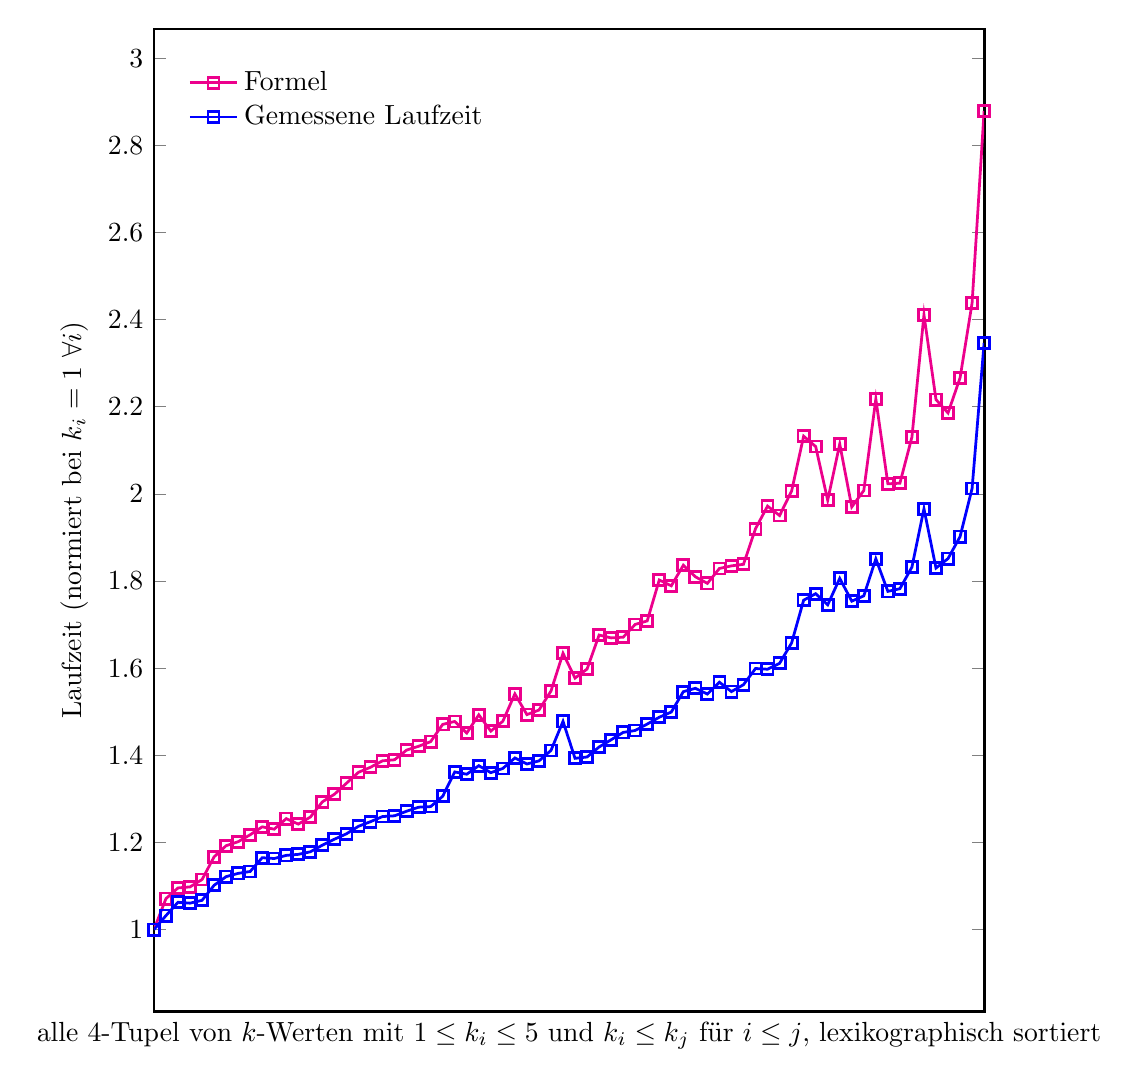
\begin{tikzpicture}
        \begin{axis}[
                xlabel = {alle 4-Tupel von $k$-Werten mit $1 \le k_i \le 5$ und $k_i \le k_j$ für $i \le j$, lexikographisch sortiert},
                ylabel = {Laufzeit (normiert bei $k_i = 1 \ \forall i$)},
                xmin = 1,
                xmax = 70,
                xmajorticks=false,
                width = \textwidth,
                height = 400pt,
                legend pos = north west,
                legend style = {draw = none},
                legend cell align = left,
                line width = 1pt,
            ]

            \addplot[color = magenta, mark = square]
            coordinates {
                    (1, 1)
                    (2, 1.0710979757195513)
                    (3, 1.0956337312770201)
                    (4, 1.0980558659801871)
                    (5, 1.1148935712138934)
                    (6, 1.1669780158585246)
                    (7, 1.1925893367387075)
                    (8, 1.2017457250065522)
                    (9, 1.217713514002541)
                    (10, 1.2358298673285073)
                    (11, 1.230570132012305)
                    (12, 1.2546783208550227)
                    (13, 1.2421716540427894)
                    (14, 1.2582606968355599)
                    (15, 1.2932616469473426)
                    (16, 1.3106291422436835)
                    (17, 1.3358668542609144)
                    (18, 1.3610552454208347)
                    (19, 1.3726236847545494)
                    (20, 1.3874292928565963)
                    (21, 1.3898045550887932)
                    (22, 1.4120323253662364)
                    (23, 1.420806693251936)
                    (24, 1.4314385754861718)
                    (25, 1.470967183593577)
                    (26, 1.4777631698932039)
                    (27, 1.4511147924955345)
                    (28, 1.4929683424271467)
                    (29, 1.4555833060998153)
                    (30, 1.4782728842829356)
                    (31, 1.5410000913052153)
                    (32, 1.4934400731302955)
                    (33, 1.5038857628628712)
                    (34, 1.5475463161560488)
                    (35, 1.6341888310284156)
                    (36, 1.5773502691896257)
                    (37, 1.5980530103927042)
                    (38, 1.6760652061461223)
                    (39, 1.6695287083889443)
                    (40, 1.6711433583422972)
                    (41, 1.700426686194625)
                    (42, 1.7085492919346918)
                    (43, 1.8024186978461607)
                    (44, 1.7890398517794515)
                    (45, 1.8362736307334504)
                    (46, 1.8099050446873453)
                    (47, 1.7945996213593973)
                    (48, 1.8289144830680806)
                    (49, 1.8348327382690706)
                    (50, 1.838415378214822)
                    (51, 1.9202299695612022)
                    (52, 1.9720192131509315)
                    (53, 1.9503324367993082)
                    (54, 2.006636656161078)
                    (55, 2.1324735486722437)
                    (56, 2.108651791874127)
                    (57, 1.9854683258448071)
                    (58, 2.1144548057613974)
                    (59, 1.9700168045378639)
                    (60, 2.007899746675162)
                    (61, 2.2177893161402236)
                    (62, 2.0231941029051845)
                    (63, 2.024552385915515)
                    (64, 2.130472790543829)
                    (65, 2.4110808212932717)
                    (66, 2.21648605664914)
                    (67, 2.18575951710838)
                    (68, 2.266287738092119)
                    (69, 2.438056280341666)
                    (70, 2.879004348902381)
                };

            \addplot[color = blue, mark = square]
            coordinates{
                    (1, 1)
                    (2, 1.032106727141481)
                    (3, 1.0627394476878842)
                    (4, 1.0607321786659445)
                    (5, 1.0672301441983756)
                    (6, 1.1016699839781903)
                    (7, 1.12156818447975)
                    (8, 1.1290462566330581)
                    (9, 1.1334523750944396)
                    (10, 1.165025014396828)
                    (11, 1.163189193205889)
                    (12, 1.1703558397523235)
                    (13, 1.1727504917278049)
                    (14, 1.1785860542345505)
                    (15, 1.1938322265498074)
                    (16, 1.2074957971526525)
                    (17, 1.2198714891907085)
                    (18, 1.2371505838544916)
                    (19, 1.2477371657508043)
                    (20, 1.25948879516128)
                    (21, 1.2612215490691463)
                    (22, 1.271711096474718)
                    (23, 1.2809960445541888)
                    (24, 1.2823822952630692)
                    (25, 1.3059688551718567)
                    (26, 1.3619311562064509)
                    (27, 1.3566344349421722)
                    (28, 1.3762691007400065)
                    (29, 1.3601954089654078)
                    (30, 1.3699413230710835)
                    (31, 1.3939229932484993)
                    (32, 1.3801580256085066)
                    (33, 1.3871628185272777)
                    (34, 1.411236257550941)
                    (35, 1.4779760510477067)
                    (36, 1.3931288422924155)
                    (37, 1.39619557161046)
                    (38, 1.419180342883475)
                    (39, 1.4357227595592452)
                    (40, 1.452590837775182)
                    (41, 1.4570705635860572)
                    (42, 1.4717664262842096)
                    (43, 1.4874283587399548)
                    (44, 1.4993435484392645)
                    (45, 1.5461192104187202)
                    (46, 1.5538247831765275)
                    (47, 1.540643911218379)
                    (48, 1.5678508748309958)
                    (49, 1.546296161807152)
                    (50, 1.5621812614531865)
                    (51, 1.599257720376162)
                    (52, 1.5976441171514473)
                    (53, 1.61113729596541)
                    (54, 1.6579489046475027)
                    (55, 1.756076957348151)
                    (56, 1.7709739026040612)
                    (57, 1.745495019609476)
                    (58, 1.806136106752739)
                    (59, 1.7538091251065155)
                    (60, 1.7660037071351078)
                    (61, 1.8510203220399712)
                    (62, 1.7762919243592523)
                    (63, 1.7824213481861442)
                    (64, 1.8320202477310212)
                    (65, 1.96584539355484)
                    (66, 1.829873906458979)
                    (67, 1.85154363339409)
                    (68, 1.9019132106278263)
                    (69, 2.012479431789328)
                    (70, 2.34633434877569)
                };

            \legend{Formel, Gemessene Laufzeit}
        \end{axis}
    \end{tikzpicture}



\end{figure}
\end{document}